\documentclass[a4paper,11pt]{article}

\usepackage{../../zyancamlec}

\def\ntripos{Mathematical Tripos}
\def\npart{III}
\def\ncourse{Symmetries, Fields and Particles}
\def\nscourse{SFP}
\def\nlecturer{B.\ Allanach}
\def\nterm{Michaelmas}
\def\nyear{2020}

\usepackage{tikz-feynhand}

\begin{document}
	\maketitlepage
	\preliminaries

	\section*{Course Information}

	Lie groups and Lie algebras are important in the construction of quantum field theories which describe interactions between known particles. Gauge theories, which describe many of the interactions in the Standard Model, rely on them. After some other preliminaries, we introduce representations in terms of square matrices. The group of rotations in three-dimensional space SO(3) is covered, along with SU(2) and the connection to angular momentum. Relativistic symmetries are discussed: in particular, the Lorentz and Poincar\'e groups and quantum fields. Lie groups and Lie algebras are covered in more generality, focusing on SU(3) as a useful example. An overview of the results of the Cartan classification of simple Lie algebras is included. Finally, gauge theory is introduced.
	
	\section*{Pre-requisites}

	Linear algebra including direct sums and tensor products of vector spaces. Special relativity and quantum theory, including orbital angular momentum theory and Pauli spin matrices.
  
	\newpage
	\tableofcontents
	\newpage
	\maintext
	\setcounter{section}{-1}
	\section{Introduction}
	\subsection{Symmetries} \lecnr{1}
	\begin{defi}
		A \emph{group} $G$ is a set $G = \{g_1, g_2, \dots\}$ with
		\begin{enumerate}
			\item A composition rule (binary operation) $*$ such that $g * g' \in G, \forall g,g' \in G$, which we shall write as $gg'$;
			\item A unique identity $e$ such that $eg=ge=g, \forall g \in G$;
			\item Associativity: $(gg')g'' = g (g'g'') := gg'g'', \forall g,g',g''\in G$;
			\item A unique inverse $\forall g\in G, \exists g^{-1}$ such that $g g^{-1} = g^{-1} g = e$.
		\end{enumerate}

		If the binary operation is commutative, we say that $G$ is \emph{abelian}.
	\end{defi}

	\begin{ex}
		Group $\mathbb{Z}_n = \{0,1,\dots,n-1\}$ with group operation being addition modulo $n$ and identity $e = 0$.

		Cyclic group $C_n = \{e^{2\pi \mathrm{i} r/n} \in \mathbb{C} : r = 0,1,\dots,n-1\}$, certain complex numbers of modulus 1, under multiplication.

		$\mathbb{Z}_n$ and $C_n$ are clearly abelian. In fact, $C_n \cong \mathbb{Z}_n$, i.e.\ they're \emph{isomorphic}, that is to say there exists a one-to-one correspondence between the elements consistent with group composition rules.
	\end{ex}

	\begin{ex}
		Symmetry groups such as the dihedral group $D_3$ \needfig{1} containing reflections along axes and rotations by $120^\circ, 240^\circ, 360^\circ$. 
	\end{ex}
	
	\begin{ex}
		\emph{Lie groups} are the generalisation to continuous symmetries, e.g.\ rotations by $\theta \in \mathbb{R}$ of a circle (``SO(2)''). Lie groups are essential to the description of particles and their interactions.
	\end{ex}

	To identify the connection between symmetries and groups, we first make the following definition.

	\begin{defi}
		A \emph{symmetry} is a transformation that leaves physical properties (e.g.\ energy, scattering probability, etc.) unchanged. They have properties:
		\begin{itemize}
			\item Symmetries can be composed: $gg' :=$ act first with $g'$, then with $g$;
			\item Doing nothing is a symmetry, $e$, the identity;
			\item A symmetry transformation $g$ can be reversed by $g^{-1}$, which is itself a symmetry.
		\end{itemize}
	\end{defi}

	From above, it is clear that the set of all symmetries forms a group. Symmetry often greatly simplifies analysis. It leads to conservation rules and constrains interactions.

	\subsubsection{Internal Symmetries}

	\emph{Internal symmetries} are properties of particles or fields themselves. 
	\begin{ex}[Colour states of a quark]
		Quarks come in three otherwise identical copies --- called `colours' ({\color{red}red}, {\color{green}green} and {\color{blue}blue}). One can continuously rotate the colours into each other, resulting in a symmetry.

		One can rotate the colour differently at different points of spacetime. In fact, one finds that one has to add a force-carrying particle to make the whole theory invariant under the symmetry. This is the gluon, which carries a colour and an anti-colour. Below is a Feynman diagram representing the fusion of a quark and an anti-quark
		\begin{center}
			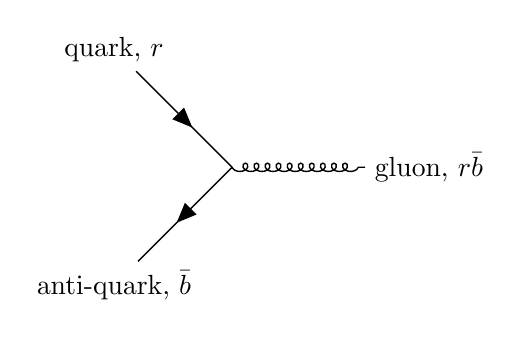
\begin{tikzpicture}
				\begin{feynhand}
					\vertex (aq) at (0,0) {anti-quark, $\bar{b}$};
					\vertex (q) at (0,3) {quark, $r$};
					\vertex [particle] (v) at (1.5,1.5);
					\vertex (f) at (4,1.5) {gluon, $r \bar{b}$};
		
					\propag [fer] (q) to [] (v);
					\propag [antfer] (aq) to [] (v);
					\propag [glu] (v) to [] (f);
				\end{feynhand}
			\end{tikzpicture}
		\end{center}

		Anti-quarks carry anti-colour $\{\bar{r}.\bar{g},\bar{b}\}$. The group structure implies that colour is conserved by interactions (i.e.\ $r \bar{b} \to r \bar{b}$ in $q \bar{q}\to g$).
	\end{ex}
	When the theory is left invariant by a symmetry transformation that's the same across whole spacetime, it's called a \emph{global symmetry}. 

	The theory of quarks, anti-quarks and gluons is called \emph{Quantum Chromodynamics} (QCD), which is a part of the Standard Model of particle physics.

	Since the colour rotations may differ at different points $(\vb x,t)$ in spacetime, it is called a \emph{local} or \emph{gauge} symmetry.

	\subsubsection{External Symmetries}

	\emph{External symmetries} involve spacetime coordinates.

	\begin{ex}
		\ 
		\begin{itemize}
			\item Translation in $(\vb x,t)$;
			\item Lorentz transformation: boosts/rotations;
		\end{itemize}
	\end{ex}

	Conserved quantities come from the group structure: e.g.\ energy, momentum, angular momentum, etc. The \emph{Poincar\'e group} consists of all these symmetries: 3 boosts, 3 rotations and 4 translations.

	Group theory has also been used in cases where the symmetries are approximate but not exact, to explain the spectrum of hadrons, for instance.

	\subsection{Particles}
	\subsubsection{Force-carriers} 
	
	Force-carriers are particles with spin 1($\hbar$) (convention $\hbar \to 1$, see QFT course).
	
	\begin{ex}
		\ 
		\begin{itemize}
			\item $g$, gluon carries colour force;
			\item $\gamma$, photons carry the electromagnetic force.
			\item $W^{\pm}, Z^0$ boson carry electroweak force that mediates radioactive decay.
		\end{itemize}
	\end{ex}

	\begin{nt}
		Bosons are integer spin particles. Fermions are half-integer spin particles.

		For spin 2, we have graviton, the force carrier of gravity. It is not seen yet because gravity is so weak.
	\end{nt}

	Force carriers belonging to a good symmetry are \emph{massless}. Those corresponding to one where the vacuum ``spontaneously'' breaks an underlying symmetry may be massive (i.e.\ $W^\pm, Z^0$ bosons, the symmetry is broken by the Higgs mechanism).

	\subsubsection{Matter Particles} 
	Matter particles are of spin $\frac{1}{2}$.
	\begin{ex}
		\
		\begin{itemize}
			\item Up quarks, electric charge $Q = + 2/3$ (choosing units where $e = 1$);
			\item Down quarks, $Q = -1/3$; 
			\item Neutrinos, $Q = 0$;
			\item Electrons, $Q = -1$.
		\end{itemize}

		They all have anti-particles, with opposite sign charge or anti-colour.
	\end{ex}

	Matter particles additionally come in 3 families, each are heavier than the last but otherwise with the same colour and charge.

	\begin{table}[H]
		\centering
		\begin{tabular}{c|c|c|c|c}		
			\hline
			Family & $Q = + 2/3$ & $Q = - 1/3$ & $Q = -1$ & $Q = 0$ \\
			\hline
			1 & up $u$ & down $d$ & electron $e$ & $e$-neutrino $\nu_e$\\
			2 & charm $c$ & strange $s$ & muon $\mu$ & $\mu$-neutrino $\nu_\mu$\\
			3 & top $t$ & bottom $b$ & tauon $\tau$ & $\tau$-neutrino $\nu_\tau$\\
			\hline
		\end{tabular}		
	\end{table}

	Anti-particles are denoted with a bar above, e.g.\ $\bar{\nu}_e, \bar{u}$, etc.

	The Standard Model explains many of these features with a QFT possessing a particular group structure of symmetries. Each particle has its own field which fills the spacetime. Quantum excitations of the fields are observed in experiments.
	\newpage

	\section{Groups: Basics} \lecnr{2}

	\subsection{Basic Concepts}

	Recall the definition of a group from last section. Here, we introduce some more definitions and facts about groups.

	\begin{defi}
		A discrete group $G$ with $n$ elements has \emph{order} $\abs{G} = n$.
	\end{defi}

	\begin{defi}
		For any group $G$, a \emph{subgroup} $H \subset G$ is naturally defined as a set of elements belonging to $G$  which is also a group itself. A \emph{proper subgroup} is when $H \neq G$, and is denoted $H < G$.
	\end{defi}

	\begin{defi}
		For any subgroup $H$, we may define an equivalence relation between $g_i, g'_i : g_i \sim g'_i \Leftrightarrow g_i = g'_i h$ for $h \in H$. Each equivalence class defines a \emph{coset} and has $\abs{H}$ elements. The cosets form a \emph{coset space} $G/H$ such that $G/H \simeq G/\sim$ and $\dim G/H = \abs{G}/ \abs{H}$. In general $G/H$ isn't a group.
	\end{defi}

	\begin{thm}[Lagrange's theorem]
		For any subgroup $H \subset G$, $\abs{H}$ divides $\abs{G}$.
	\end{thm}

	\begin{defi}
		The \emph{index} of subgroup $H$ in $G$ is the number of cosets in $G/H$, denoted $G:H = \abs{G}/\abs{H}$.
	\end{defi}

	\begin{defi}
		A \emph{normal}, or \emph{invariant} subgroup is a subgroup $H \subset G$ such that
		\[
			g H g^{-1} = H \quad \forall g \in G.
		\]
		This is denoted $H \triangleleft G$ (or $G \triangleright H$).
	\end{defi}

	\begin{prop}
		For a normal subgroup $H$ of $G$, $G/H$ becomes a group.
	\end{prop}
	\begin{proof}[Proof Sketch]
		For $g_i' = g_i h_i, g_j' = g_j h_j$ with $h_i, h_j \in H$, then $g_i' g_j' = g_i g_j h$ for some $h \in H$. (Try to complete the proof.)
	\end{proof}
	\begin{cor}
		For an abelian group, all subgroups are normal subgroups.
	\end{cor}

	\begin{defi}
		A group is \emph{simple} if the only normal subgroups are $G$ and the trivial subgroup formed by the identity $e$ itself.
	\end{defi}

	\begin{defi}
		The \emph{centre} of a group $G$, denoted $\mathcal{Z}(G)$, is the set of all elements which commute with all elements of $G$. It is an abelian, normal subgroup.
	\end{defi}
	
	\begin{defi}
		For two groups $G_1$ and $G_2$, we may define a \emph{direct product group} $G_1 \times G_2$ formed by pairs of elements $\{(g_1,g_2)\}$ belonging to $(G_1,G_2)$, defined by the rules 
		\begin{itemize}
			\item $(g_1, g_2)(g_1',g_2') = (g_1 g_1', g_2 g_2')$;
			\item $(g_1, g_2)^{-1} = (g_1^{-1}, g_2^{-1})$;
			\item $e = (e_1,e_2)$.
		\end{itemize}

		So long as it is clear which elements belong to $G_1$ and which to $G_2$, we may write the elements of $G_1 \times G_2$ as $g_1 g_2$ or $g_2 g_1$.
	\end{defi}

	\begin{cor}
		For finite groups $\abs{G_1 \times G_2} = \abs{G_1}\abs{G_2}$.
	\end{cor}

	\subsection{Cyclic, Dihedral and Permutation Groups}
	\subsubsection{Cyclic Groups}

	Clearly $\mathbb{Z}_n$ is abelian. For $p$ prime, $\mathbb{Z}_p$ has no subgroups. $p$ has no divisors, hence $\mathbb{Z}_p$ is simple.

	\begin{prop}
		If $n = pq$ then $\mathbb{Z}_p$ and $\mathbb{Z}_q$ are normal subgroups of $\mathbb{Z}_n$ and $\mathbb{Z}_{pq} / \mathbb{Z}_p \simeq \mathbb{Z}_q$. If $p,q$ are co-prime (i.e.\ no common factors), then $\mathbb{Z}_{pq} \simeq \mathbb{Z}_p \times \mathbb{Z}_q$.
	\end{prop}

	\subsubsection{Dihedral Groups}

	\begin{defi}
		The \emph{dihedral group} $D_n$ of order $2n$, is the symmetry groups of a regular $n$-sided polygon, formed by rotations $a$ through angles $2\pi r / n, r = 0, \cdots ,n-1$, together with reflections$b$. In general,
		\[
			D_n = \{a^r, a^rb : (r = 0, \cdots, n-1; a^0 = a^n =e; b^2 = e; ab = ba^{r-1})\}.
		\]
	\end{defi}
	
	For any $r$, we have $(a^r b)^2 = e$.

	For $n>2$, the group is non-abelian since $ab \neq ba $. 

	It is an easy observation that
	\[
		D_2 \simeq \mathbb{Z}_2 \times \mathbb{Z}_2
	\]
	
	\subsubsection{Permutation (or Symmetric) Groups}
	\begin{defi}
		The \emph{permutation group} $S_n$ acting on $n$ objects, is the group of all permutations of these $n$ objects. It has $\abs{S_n} = n!$.
	\end{defi}

	\begin{ex}
		$S_3 \simeq D_3$: symmetry group of equilateral triangle under permutations of vertices.
	\end{ex}

	\begin{defi}
		$A_n$, the \emph{alternating group}, is a normal subgroup of $S_n$ formed by the even permutations. $\abs{A_n} = n! / 2$.
	\end{defi}

	\begin{cor}
		For $n \geq 5$, $A_n$ is simple.
	\end{cor}

	\begin{prop}
		\[
			S_n / A_n \simeq \mathbb{Z}_2.
		\]
	\end{prop}

	Also, note $A_3 \simeq \mathbb{Z}_3$.

	The elements of the permutation group can be decomposed into \emph{cycles}. Acting on $\{1,2,\cdots, n\}$, 
	\begin{itemize}
		\item 2-cycle $(ij)$ with $i\neq j$, swaps $i$ and $j$;
		\item 3-cycle $(ijk)$ with $i\neq j \neq k$, takes $i \to j \to k \to i$;
		\item ... 
	\end{itemize}
	Thus we generalise to the following.

	\begin{defi}
		A \emph{$p$-cycle} $(i_1 i_2 \cdots i_p)$ for all $i_j$ different with $p \leq n, 1 \leq i_j \leq n$ generates cyclic permutations of $\{i_1, \cdots, i_p\}$. 
	\end{defi}

	Note that $(i_1 i_2 \cdots i_p)^p = e$.

	For any one of the $\rk{n}{p}$ choices of $\{i_j\}$, there exists $(p-1)!$ choices for the $p$-cycle involving $\{i_j\}$, since any $p$-cycle is invariant under cyclic permutations.

	For distinct $i,j,k,l$
	\[
		(ij)(kl) = (kl)(ij) \quad \text{and} \quad (ij) (jk) = (ijk).
	\]
	
	\begin{prop}
		The action of some $g \in S_n$ can be decomposed into cycles.
	\end{prop}

	\begin{proof}
		Consider an arbitrary $i \in \{1,2,\cdots, n\}$ and act $g$ on $i$ by $g^r i, r = 1,2,\cdots$ For some minimal $p$, we have $g^p i = i$. The action of $g$ then generates a $p$-cycle $(i_1 \cdots i_p)$. 
	
		Now we pick $j\in \{1,2,\cdots,n\} \backslash \{i_1, \cdots, i_p\}$ acting repeatedly with $g$ generates a new $q$-cycle $(j_1 \cdots j_q)$ for some $q$ and $j_1 = j$. Continuing, any element of $\{1,2,\cdots,n\}$ belongs to some cycle.
	\end{proof}

	If $gk = k$, then the element belongs to the 1-cycle $(k)$.

	We may denote $g$ as $g_{(i_1 \cdots i_p)(j_1 \cdots j_q)\cdots}$, $e = e_{(1)(2)\cdots(n)}$ and $g^{-1} = g_{(i_p \cdots i_1)(j_q \cdots j_1)\cdots}$.
	
	If $h$ corresponds to a permutation $\sigma$ where $\sigma \{1,2,\cdots,n\} = \{\sigma(1),\sigma(2),\cdots, \sigma(n)\}$, then
	\[
		h g_{(i_1 \cdots i_p)(j_1 \cdots j_q)\cdots}h^{-1} = g_{(\sigma(i_1)\cdots \sigma(i_p))(\sigma(j_1)\cdots \sigma(j_q))\cdots}.
	\]

	\subsection{Orbit Stabiliser Theorem}

	Now we introduce \emph{orbit stabiliser theorem}, which applies when a group $G$ acts an a space $X = \{x\}$ such that $\forall g \in G, x \to gx$. 

	\begin{defi}
		For any particular $x \in X$, the \emph{stabiliser group} or \emph{little group} $G_x$ is defined by those elements of $G$ which leave $x$ invariant, i.e.\ 
		\[
			G_x = \{h : h\in G, h x = x\}.
		\]
		a subgroup of $G$.
	\end{defi}

	\begin{defi}
		The \emph{orbit} of $x$ is the set of points in $X$ obtained by the action of $G$, 
		\[
			O_x = \{x' : x' = g x, \forall g \in G\}.
		\]
	\end{defi}

	\begin{thm}[Orbit stabiliser theorem]
		$O_x$ can be identified with $G / G_x$. For a finite group $G$, $\dim O_x = \abs{G}/\abs{G_x} \in \mathbb{Z}$ by Lagrange's theorem. For $x' \in O_x$, $G_{x'} \simeq G_x$. In general, the space $X$ can be decomposed into orbits under the action of $G$.
	\end{thm}

	\begin{hint}
		$G_{x'} \simeq G_x$ since $hx = x$ and $x' = gx$, giving $h'x' = x'$ for $h' = ghg^{-1}$. 
	\end{hint}
	
	\subsection{Automorphisms and Semi-Direct Product} \lecnr{3}

	\begin{defi}
		An \emph{automorphism} of a group $G = \{g_i\}$ is defined as a mapping between elements $g_i \to \phi(g_i)$ such that the product rule is preserved, i.e. 
		\[
			\phi(g_i) \phi(g_j) = \phi(g_i g_j), \quad g_i, g_j \in G
		\]
		and $G_\phi = \{\phi(g_i)\} \simeq G$. It must have $\phi(e) = e$ and $\phi(g^{-1}) = \phi(g)^{-1}$. 

		For any fixed $g \in G$ we may define an \emph{inner automorphism} by
		\[
			\phi_g (g_i) = g g_i g^{-1}.
		\]
		
		Automorphisms not of this form are called \emph{outer automorphisms}.
	\end{defi}

	\begin{prop}
		The set of all automorphisms forms a group $\Aut G$, which should include $G / \mathcal{Z}(G)$ as a normal subgroup.
	\end{prop}
	
	\begin{prop}
		For any abelian group, there are no non-trivial inner automorphisms, but there can be outer ones.
	\end{prop}

	\begin{ex}
		For $\mathbb{Z}_3$, take $\{e, a, a^2\} \to \{e, a^2, a\}$. In this case, $\Aut \mathbb{Z}_3 = \mathbb{Z}_2$ and $\mathbb{Z}_3 / \mathcal{Z}(\mathbb{Z}_3) = \{e\}$, the trivial one-element group. 
	\end{ex}

	\begin{lem}
		If $H \subset \Aut G$ such that for any $h\in H$ and any $g \in G$, we have
		\[
			g \xrightarrow{h} \phi_h (g)
		\]
		with 
		\[
			\phi_h (g_1) \phi_h (g_2) = \phi_h (g_1 g_2)
		\]
		and
		\[
			\phi_{h_1}(\phi _{h_2} (g)) = \phi _{h_1 h_2} (g)
		\]
		also $\phi_h (e) = e, \phi_e (g) = g, \phi_{h^{-1}} (g) = \phi_h ^{-1} (g)$. 
	\end{lem}

	\begin{defi}
		The above proposition allows us to define a new group called the \emph{semi-direct product} of $H$ with $G$, denoted as $H \ltimes G$. As with the direct product, this is defined in terms of pairs of elements $(h,g)$ belonging to $(H,G)$ but with a less trivial product rule
		\begin{align*}
			(h,g) (h',g') &= (hh', g \phi_h (g')),\\
			(h,g)^{-1} & = (h^{-1}, \phi _{h^{-1}} (g)).
		\end{align*}
	\end{defi}

	\begin{cor}
		The above product rule of $H \ltimes G$ implies
		\[
			(h,e)(e,g)(h,e)^{-1} = (e, \phi_h(g)).
		\]
		
	\end{cor}

	It's often convenient to write the elements of $H \ltimes G$ as $(h,g) \to hg : = \phi_h(g)h$ as an abbreviation.

	\begin{prop}
		$G$ is a normal subgroup of $H \ltimes G$.
	\end{prop}
	\begin{proof}[Proof sketch]
		\[
			(h,g)(e,g')(h,g)^{-1} = (e, g \phi_h(g') g^{-1})
		\]
		for any $g,g' \in G$ and $h\in H$ so that
		\[
			H \simeq (H \ltimes G / G).
		\]
	\end{proof}

	\begin{ex}
		$D_n \simeq \mathbb{Z}_2 \ltimes \mathbb{Z}_n$, where
		\[
			\mathbb{Z}_2 = \{e, b : b^2 = e\}
		\]
		and
		\[
			\mathbb{Z}_n = \{a^r: r= 0, \cdots, n-1, a^n = e\}
		\]
		and we define for any $g = a^r \in \mathbb{Z}_n$,
		\[
			\phi_b (g) = g^{-1} = b g b^{-1}.
		\]
	\end{ex}

	\subsection{Conjugacy Classes}

	\begin{defi}
		If $g_j = g g_j g^{-1}$ for some $g \in G$, then $g_i$ is \emph{conjugate} to $g_j$, written as $g_i \sim g_j$. The equivalence relation $\sim$ divides $G$ into \emph{conjugacy classes}
		\[
			\mathcal{C}_r = \{g_i: g_i \sim g_i' = g g_i g^{-1}, g \in G\}.
		\]
	\end{defi}

	The identity $e$ is in a conjugacy class by itself. For an abelian group, all elements have their own conjugacy class.

	Elements of a conjugacy class have similar properties, e.g.\ $g_i^n = e$ for the same $n$ for all $g_i \in \mathcal{C}_r$.

	\begin{ex}
		For $S_3 = \{e, a, a^2, b, ab, a^2 b\}$ with $b = (1\ 2), a = (1\ 2\ 3)$, there exist 3 conjugacy classes
		\[
			\{e\}, \quad \{a, a^2\}, \quad \{b, ab, a^2 b\}.
		\]
		
	\end{ex}

	\begin{nt}
		If we have $a ^{n} = e$, then $g a^n g^{-1} = e$ so that $(g a g^{-1})^n = e$, too. 
	\end{nt}

	\subsection{Normaliser, Centraliser, Commutator}

	\begin{defi}
		For a subgroup $H \subset G$, the elements $g \in G$ such that $g h g^{-1} \in H, \forall h \in H$ (we write this as $gHg^{-1} = H$) form a subgroup of $G$ which contains $H$ itself, called the \emph{normaliser} of $H$ in $G$, denoted as $N_G(H)$.
	\end{defi}
	\begin{cor}
		Clearly, $H \triangleleft N_G(H)$.
	\end{cor}

	\begin{defi}
		The subgroup of $G$ formed by elements such that $g h g^{-1} = h, \forall h \in H$ forms the \emph{centraliser} $C_G(H)$.
	\end{defi}

	\begin{cor}
		Necessarily, $C_G(H) \subset N_G(H)$.
	\end{cor}

	\begin{defi}
		For any $g \in G, h \in G$, 
		\[
			[g,h] : = g^{-1} h^{-1} g h
		\]
		is the \emph{commutator} of $g$ and $h$. 
		
		We say $g$ is \emph{abelian}, if
		\[
			[g,h] = e, \quad \forall h\in G.
		\]

		More generally, if $[g,h] = e$, we say that $g$ and $h$ \emph{commute}.
	\end{defi}

	\begin{cor}
		In general
		\[
			[g,h]^{-1} = [h,g]
		\]
		and for any $g' \in G$,
		\[
			g' [g,h] g'^{-1} = [g' g g'^{-1}, g' h g'^{-1}].
		\]
	\end{cor}

	\begin{defi}
		The \emph{commutator subgroup} or \emph{derived subgroup} of $G$, denoted $G' = [G,G]$, is formed by arbitrary products of commutators.
	\end{defi}

	\begin{cor}
		From above,
		\[
			g[G,G]g^{-1} = [G,G] \quad \forall g \in G
		\]
		so $[G,G]$ is a normal subgroup.
	\end{cor}

	\begin{cor}
		For any $g_1, g_2 \in G$, we have
		\[
			g_1 g_2 = g_2 g_1 [g_1, g_2]
		\]
		so $G/ [G,G]$ is abelian.
	\end{cor}

	\begin{defi}
		A group is \emph{perfect} if $G = [G,G]$.
	\end{defi}

	\newpage

	\section{Matrix Groups}

	Any set of non-singular matrices which is closed under matrix multiplication forms a \emph{matrix group}. We choose $e$ to be identity matrix, inverse to be the matrix inverse. Many groups are defined in terms of matrices.

	\begin{defi}
		The \emph{real general linear group} $\GL(n,\mathbb{R})$ is the set of all real $n \times n$ non-singular matrices (i.e.\ $\det M \neq 0, \forall M \in \GL(n,\mathbb{R})$). Its real dimension is $n^2$.

		Similarly, we can define the \emph{complex} general linear group $\GL (n,\mathbb{C})$, which has real dimension $2 n^2$.
	\end{defi}

	\begin{defi}
		The real \emph{special linear group} $\SL(n,\mathbb{R})$ is the set of all real non-singular $n \times n$ matrices with $\det M = 1, \forall M \in \SL(n,\mathbb{R})$. It has real dimension $n^2 - 1$.
	\end{defi}

	\subsection{Continuous Matrix Groups of Interest}

	\begin{enumerate}
		\item $\Og(n)$, real orthogonal $n\times n$ matrices such that \begin{equation}
			M^T M = I, \quad \forall M \in \Og(n).
			\label{eq:2.1.1}
		\end{equation}
		
		For $\SO(n)$, we have the condition $\det = 1$ as well.

		To find the (real) dimension of such groups, note that a general $n \times n$ real matrix has $n^2$ parameters. A symmetric one has $\frac{n}{2} (n+1)$ free entries. $M^T M$ is a symmetric matrix, so (\ref{eq:2.1.1}) imposes $\frac{n}{2}(n+1)$ constraints. So, $\Og(n)$ has $\frac{1}{2} n (n-1)$ parameters. So does $\SO(n)$ as the defining relation already gives $\abs{\det M}=1$.
		
		If $v,v'$ belong to the $n$-dimensional representation space (to be defined) of $\Og(n)$ or $\SO(n)$, then the scalar product $v'^T v$ is invariant under
		\[
			v \to Mv, \quad v' \to Mv'.
		\]
		\item $\U(n)$, the complex unitary $n\times n$ matrices with \begin{equation}
			M^\dagger M = I, \quad \forall M \in \U(n).
			\label{eq:2.1.2}
		\end{equation} 

		A Hermitian complex matrix has $n^2$ real parameters. $M^\dagger M$ is Hermitian, then (\ref{eq:2.1.2}) contains $n^2$ constraints. Thus in $\U(n)$, we have $2n^2 - n^2 = n^2$ real parameters. 
		
		(\ref{eq:2.1.2}) implies $\abs{\det M} = 1$, so imposing $\det M = 1$ provides one additional constraint, giving the special unitary group, $\SU(n)$, with $n^2 - 1$ real parameters.

		The $\U(n)$ invariant product for $n$-dimensional complex vectors $v,v'$ is $v'^\dagger v$.
	\end{enumerate}

	\begin{ex}
		$\SO(2) \simeq \U(1)$ since a general $\SO(2)$ matrix
		\[
			\begin{pmatrix}
				\cos \theta & \sin \theta\\
				-\sin \theta & \cos \theta
			\end{pmatrix}
		\]
		with $0 \leq \theta \leq 2 \pi$ is in one-to-one correspondence with a general element of $\U(1)$: $e ^{\mathrm{i} \theta}$, $0 \leq \theta \leq 2 \pi$.

		Topologically, $\U(1) \simeq S^1$.

		For $\SU(2)$,
		\[
			g = \begin{pmatrix}
				\alpha & \beta\\
				-\beta^* & \alpha^*
			\end{pmatrix}
		\]
		where $\abs{\alpha}^2 + \abs{\beta}^2 = 1$.

		Write 
		\[
			\alpha = a + \mathrm{i} b, \quad \beta = c + \mathrm{i} d
		\]
		we get
		\[
			a^2 + b^2 + c^2 + d^2 = 1
		\]
		i.e.\ the 3-sphere $S^3$.
	\end{ex}

\end{document}